% LaTeX poster using beamerposter class (3-column layout)
\documentclass[final]{beamer}

% Poster theme and packages
\usepackage[size=a0,scale=1.0]{beamerposter}
\usepackage{amsmath, amssymb}
\usepackage{graphicx}
\usepackage{xcolor}
\usepackage{multicol}
\usepackage{tikz}
\usetikzlibrary{positioning} % <-- added for 'of=' syntax in tikz
\usepackage[utf8]{inputenc} % Ensure unicode compatibility
\usepackage{lmodern} % Better font rendering for large fonts

% Custom NYU Violet color and styling
\definecolor{nyuviolet}{RGB}{87, 0, 140}
\setbeamercolor{block title}{bg=nyuviolet, fg=white}
\setbeamercolor{block body}{bg=white, fg=black}
\setbeamerfont{block title}{series=\bfseries}

%% FOR colors used in equations:
\definecolor{myred}{RGB}{200,0,0}
\definecolor{myblue}{RGB}{0,0,180}
% define a big fat red todo command
\newcommand{\todo}[1]{\textcolor{myred}{\textbf{TODO:} #1}}

% Title and authors
\title{On the Difficulty of Training Recurrent Neural Networks}
\author{Razvan Pascanu, Tomas Mikolov, Yoshua Bengio}
\institute{ICML 2013}

% Document
\begin{document}

\begin{frame}[t]
%%%%%%%%%%%%%%%%%%%%%%%%%%%%%%%%%%%% Title Block %%%%%%%%%%%%%%%%%%%%%%%%%%%%%%%%%%%%%%%%%%%%%%%%%%%%%%%%
    \begin{columns}[t,totalwidth=\textwidth]
    \begin{column}{0.66\textwidth}
      \vspace{1em}
      {\centering
        {\veryHuge\bfseries On the Difficulty of Training RNNs}\\[0.5em]
        {\Huge R. Pascanu, T. Mikolov, Y. Bengio}\\[0.5em]
        {\Large\itshape ICML 2013}\\
      }
    \end{column}
    \begin{column}{0.33\textwidth}
      \flushright
      \Large \textit{Presented by OUR NAMES: Hanna M. Dettki}
    \end{column}
  \end{columns}
  \vspace{2em}

  % Main body columns
  \begin{columns}[t,totalwidth=\textwidth]

    %%%%%%%%%%%%%%%%%%%%%%%%%%%%%%%%%%%% Column 1 %%%%%%%%%%%%%%%%%%%%%%%%%%%%%%%%%%%%%%%%%%%%%%%%%%%%%%%%
    \begin{column}{0.33\textwidth}
      \begin{block}{1. Introduction \& Background} \todo{}

        \textbf{1.1 Context \& Motivation}
            \begin{itemize}
            \item \textbf{Importance of sequence modeling}
            \begin{itemize}
                \item e.g., language, time-series in finance
            \end{itemize}

            \item Identifying gradient problems (Bengio et al., 1994)
            \begin{itemize}
                \item \textbf{Vanishing gradient problem}: impossible to learn long-term dependencies
                \item \textbf{Exploding gradient problem}: numerical instabilities $\rightarrow$ unstable training
            \end{itemize}

            \item $\rightarrow$ Why stable gradient flow is critical for learning temporal dependencies (paper's contribution)
            \end{itemize}




        \vspace{1em}


        \textbf{1.2 Schematic \& formal def. of RNN}

            \begin{tikzpicture}[node distance=2.5cm, thick, >=latex, every node/.style={scale=1.5}, xshift=-1cm]
            % Nodes
            \node[draw, minimum height=1.5cm, minimum width=0.8cm] (input) {$u_t$};
            \node[draw, right=of input, minimum height=1.5cm, minimum width=0.8cm] (rnn) {$x_t$};
            \node[right=of rnn] (error) {$\mathcal{E}_t$};
            
            % Arrows
            \draw[->, line width=1.5pt] (input) -- (rnn);
            \draw[->, line width=1.5pt] (rnn) -- (error);
            
            % Recurrent loop (from right to left, meeting top corners)
            \draw[->, orange, line width=2pt]
                ([xshift=3pt,yshift=3pt]rnn.north east)
                to[out=45,in=135,looseness=1.2]
                ([xshift=-3pt,yshift=3pt]rnn.north west);
            
            % Label
            \node[below=0.5cm of input] {Fig. 1};
            \end{tikzpicture}
        % \end{center}
    

        \vspace{0.5em}
        \begin{align*}
          x_t &= F(x_{t-1}, u_t, \theta) && \text{(1) General} \\
          x_t &= \textcolor{orange}{W_{\text{rec}}} \, \sigma(x_{t-1}) + W_{in} u_t + \mathbf{b} && \text{(2)}
        \end{align*}

        \vspace{0.5em}
        \small
        where $u_t$: input, $x_t$: state, $t$: time step, $\mathbf{b}$: bias, $\mathcal{E}_t = \mathcal{L}(x_t)$ (error)

        \vspace{0.5em}
        \textcolor{orange}{\textbf{The recurrent connections}} in the hidden layer allow information to persist from one input to another.

        \vspace{1em}
        \textbf{1.3 Training RNNs: Backprop Through Time (BPTT) on Unrolled RNN}\\
        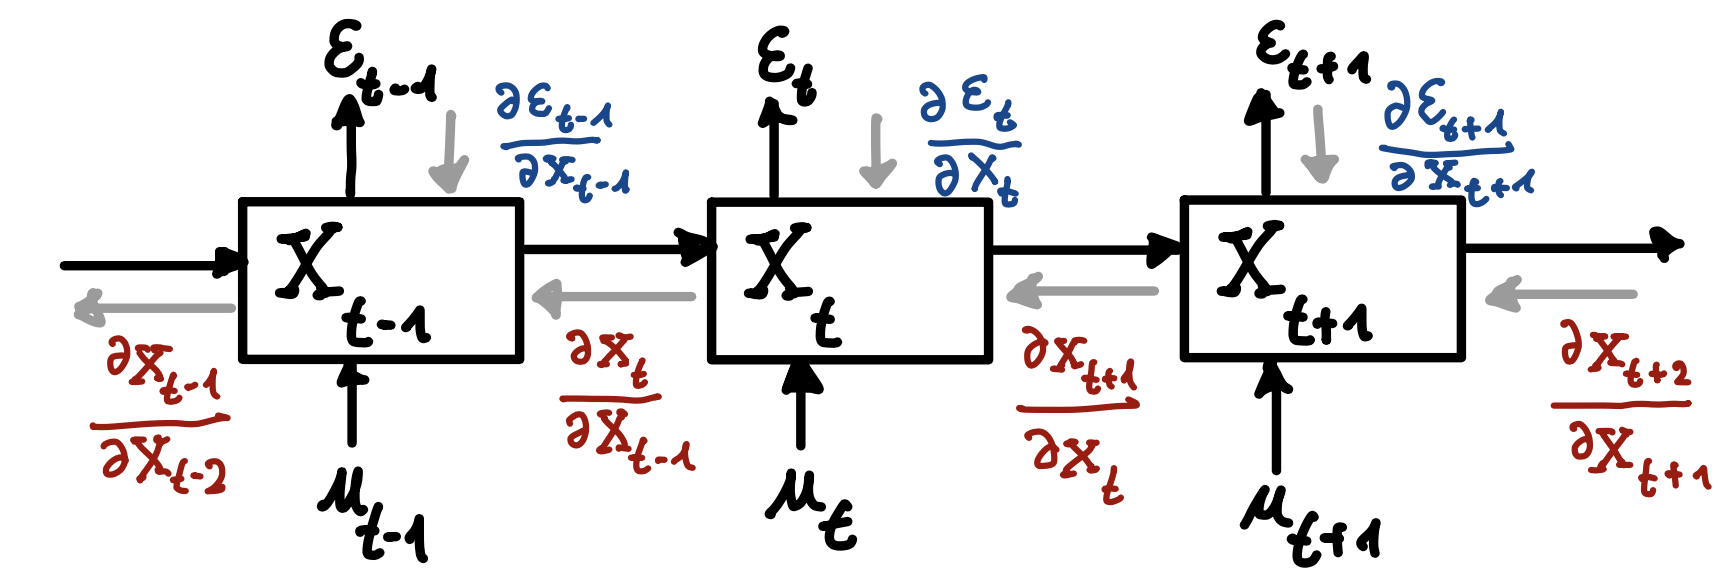
\includegraphics[width=0.95\linewidth]{figures/2_fig.png}\\[0.5em]
        Fig. 2: Unrolled RNN


        \vspace{0.3em}
        %\small
        \begin{align*}
          \textcolor{myblue}{\frac{\partial \mathcal{E}}{\partial \theta}} &=
          \sum_{t=1}^{T} \frac{\partial \mathcal{E}_t}{\partial \theta} \hspace{2em} \text{(3)} \\[0.5em]
          \frac{\partial \mathcal{E}_t}{\partial \theta} &=
          \sum_{k=1}^{t} 
          \left( {\frac{\partial \mathcal{E}_t}{\partial x_t}} 
          \textcolor{myred}{\frac{\partial x_t}{\partial x_k}}
          \frac{\partial^+ x_k}{\partial \theta} \right) \hspace{2em} \text{(4)} \\[0.5em]
          \textcolor{myred}{\frac{\partial x_t}{\partial x_k}} &=
          \prod_{i=k+1}^{t}
          \textcolor{orange}{W_{\text{rec}}}^\top \cdot \text{diag}\left(\sigma'(x_{i-1})\right) \hspace{2em} \text{(5)}
        \end{align*}
        
        \vspace{0.5em}
        where $\frac{\partial^+ x_k}{\partial \theta}$ denotes the “immediate” partial derivative (treating $x_{k-1}$ as constant).
        
        \vspace{0.5em}
        \textcolor{myblue}{Blue}: total gradient over time.
        \quad
        \textcolor{myred}{Red}: temporal error contribution.

      \end{block}
    \end{column}



    %%%%%%%%%%%%%%%%%%%%%%%%%%%%%%%%%%%% Column 2 %%%%%%%%%%%%%%%%%%%%%%%%%%%%%%%%%%%%%%%%%%%%%%%%%%%%%%%%
        \begin{column}{0.33\textwidth}
            \begin{block}{2. The Problem} \todo{}
        
            \textbf{2.1 Vanishing Gradient problem (VG)}\\[0.3em]
            \textit{Sufficient condition:}
            \[
                \textcolor{orange}{\lambda_1} < \frac{1}{\gamma}
            \]
            where: $\lambda_1$: largest singular value of $W_{\text{rec}}$\\
            \phantom{where: }$\gamma$: bound on derivative of activation function\\[0.3em]
            (proof: see eq. 6 \& 7)
        
            \vspace{1em}
            \textbf{2.2 Exploding Gradient problem (EGs)}\\[-0.2em]
            \begin{itemize}
                \item gradients grow exponentially during backprop
                \item \textit{Necessary condition:}
                \[
                \lambda_1 > \frac{1}{\gamma}
                \]
            \end{itemize}
        
            \vspace{1em}
            \textbf{2.2.1 Dynamical systems interpretation:}
            \begin{itemize}
                \item EGs create steep wall-like structures 
                    that are perpendicular to exploding direction 
                    in error surface
            \end{itemize}
        
            \vspace{2em}
            \begin{center}
                \fbox{\parbox{0.9\linewidth}{\centering \vspace{10em} \textit{placeholder figure} \vspace{2em}}}\\[0.3em]
                Fig. 3
            \end{center}
        
            \end{block}
        \end{column}
  

    % %%%%%%%%%%%%%%%%%%%%%%%%%%%%%%%%%%%% Column 3 %%%%%%%%%%%%%%%%%%%%%%%%%%%%%%%%%%%%%%%%%%%%%%%%%%%%%%%%
    % \begin{column}{0.33\textwidth}
    %   \begin{block}{3. Solution \& Experiments}
    %     % TODO: fill in this section
    %   \end{block}
    % \end{column}

    %%%%%%%%%%%%%%%%%%%%%%%%%%%%%%%%%%%% Column 3 %%%%%%%%%%%%%%%%%%%%%%%%%%%%%%%%%%%%%%%%%%%%%%%%%%%%%%%%
\begin{column}{0.33\textwidth}
    \begin{block}{3. Solution \& Experiments}
  
      \textbf{3.1 Gradient Clipping}
      \begin{itemize}
        \item see Fig. 3 for \textit{motivation}
        \item Pseudo-code for norm-clipping
        \item \todo{}
      \end{itemize}
  
      \vspace{0.5em}
      \textbf{3.2 VG-Regularization}
      \begin{itemize}
        \item see paper eq. 9 \& 10
        \item  \todo{}
      \end{itemize}
  
      \vspace{0.5em}
      \textbf{3.3 MSGD-CR}
        \begin{itemize}
            \item \todo{}
            \item  (combines 3.1 \& 3.2)
            
    \end{itemize}
  
      \vspace{0.5em}
      \textbf{3.4 Initialization Strategies}
      \begin{itemize}
        \item see experiments in Sec. 4
      \end{itemize}
  
      \vspace{1em}
      \begin{center}
        \fbox{\parbox{0.9\linewidth}{\centering \vspace{10em} \textit{placeholder figure} \vspace{2em}}}
        \\[0.3em]
        Fig. 4
      \end{center}

      \begin{center}
        \fbox{\parbox{0.9\linewidth}{\centering \vspace{10em} \textit{placeholder figure} \vspace{2em}}}
        \\[0.3em]
        Fig. 5
      \end{center}
  
    \end{block}
  
    \vspace{1em}
  
    \begin{block}{4. Relevance today \& SOTA techniques} \todo{}
      \begin{itemize}
        \item Clipping still relevant!
        \item Instead of regularization:
        \begin{itemize}
          \item residual connections
          \item gradient checkpointing
          \item gating mechanisms
          \item layer normalization
          \item attention mechanism
          \item positional encoding
        \end{itemize}
      \end{itemize}
    \end{block}
  \end{column}
  

  \end{columns}

\end{frame}

\end{document}
